\chapter{Spintronique moléculaire}

\section{Spintronique et Électronique moléculaire}
La micro-électronique a su évoluer au gré des développements scientifiques. Elle a tout d'abord su tirer avantage des travaux sur la magnéto-résistance géante au travers d'une nouvelle discipline : la spintronique. Pendant presque deux décennies, celle-ci a permis d'améliorer de plusieurs ordres grandeurs les capacités de stockage des composants électroniques. Plus récemment, le développement de molécules organiques semi-conductrices~\cite{Tsumura1986,Horowitz1990,Lin1997} a poussé encore une fois l'électronique dans une nouvelle voie, celle de l'électronique moléculaire.

Ces deux évolutions pourraient bientôt fusionner pour tirer avantage des concepts issues de la spintronique et du formidable potentiel de l'électronique moléculaire.

\subsection{La spintronique}
La spintronique est une branche de l'électronique où, en plus de la charge, le degré de liberté du spin de l'électron est utilisé. Elle est notamment à l'origine des avancés technologiques les plus récentes telles que la MRAM~(Magnetic Random Access Memory) ou bien encore les têtes de lecture des disques durs~(cf Fig.\ref{SpinValve}.\textbf{b}). Mais le dispositif le plus célèbre, à la base des technologies précédemment citées, reste sans doute la vanne de spin. Celui-ci permet de filtrer les électrons en fonction de l'orientation de leur spin (soit \textit{up}, soit \textit{down}), autorisant un couplage direct entre magnétisme et courant électrique. La découverte du phénomène de magnétorésistance géante~(cf Fig.\ref{SpinValve}.\textbf{a}), à l'origine de ce filtrage, a d'ailleurs value à ses découvreurs, Albert Fert~\cite{Baibich1988} et Peter Grünberg~\cite{Gruenberg1986}, le prix Nobel de Physique en 2007.

\begin{figure}
\centering 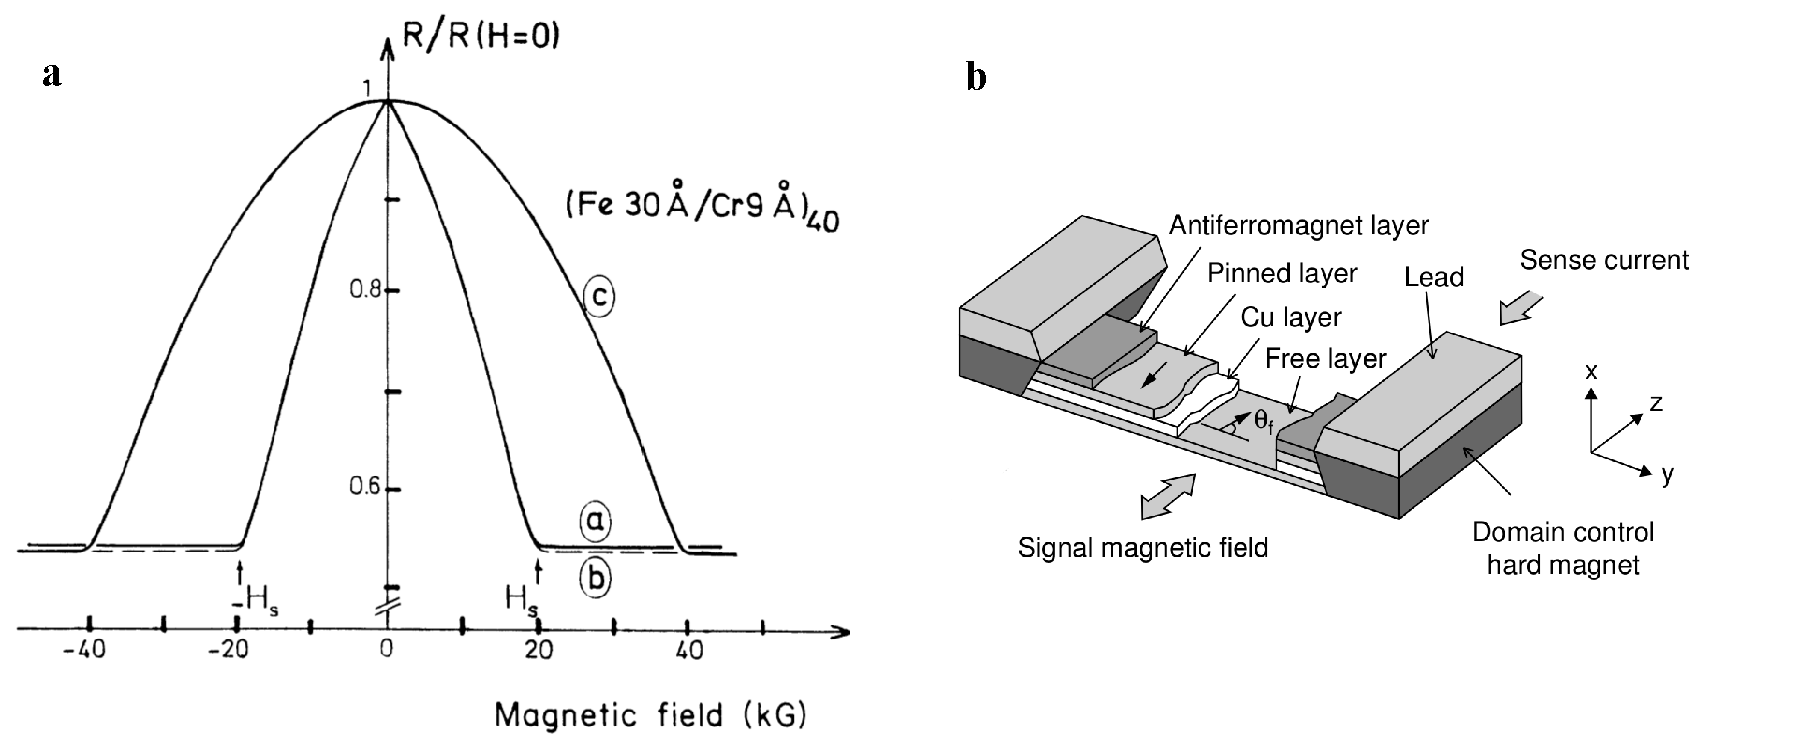
\includegraphics[scale=0.45]{Spintronique/SpinValve/SpinValve.pdf}
\caption{\textbf{a} : mesure de la résistance d'une valve de spin mettant en évidence la magnéto-résistance géante~(extrait de ~\cite{Baibich1988}).  \textbf{b} : Schéma d'une tête de lecture de disque dur dont le fonctionnement est basé sur le phénomène de magnéto-résistance~(extrait de~\cite{Hitoshi2001}).}
\label{SpinValve}
\end{figure}



La spintronique, dans ses applications, reste cependant cantonnée au stockage de  l'information~\cite{Awschalom2007}. Des propositions de transistors de spin, directement commandés par le spin électronique, ont pourtant été faites~\cite{Datta1990}, et certains dispositifs ont également été réalisés~\cite{Johnson1996,Huang2007}. Mais de tels systèmes n'ont pas, pour l'instant, quitté les laboratoires.

De plus, elle se heurte aux défis de la miniaturisation, qui ne lui sont pas spécifiques, mais qui se posent à l'ensemble de l'électronique. Le salut des futurs dispositif pourrait bien se trouver dans l'électronique organique.

\subsection{L'électronique organique}
Devant le besoin toujours plus grand de miniaturisation des dispositifs, les chercheurs et les industriels se sont vite rendus compte des limites des techniques de fabrication traditionnelles. Elles consistent à partir d'un matériau massif, et de graver en son sein, les structures nanométriques nécessaires à la production de l'électronique actuelle. C'est l'approche dite``\textit{Top-Down}"

Devant les progrès récents de la chimie organique, une seconde solution est apparue, faisant appel à cette dernière  pour produire les objets de petite taille et les disposer de manière contrôlée : c'est l'approche dite ``\textit{Bottom-Up}". Dans cette approche, deux caractéristiques des molécules sont exploités : leur capacité à s'auto-assembler, c'est à dire à adopté une configuration précise ``programmée" à travers les ligands; la possibilité de fabriquer des milliards de molécules toutes identiques, avec une grande pureté. 

L'histoire de l'électronique moléculaire est cependant relativement récente. Comme le rappelle G. Horowitz dans~\cite{Klauk2007}, l'industrie s'est finalement intéressée à ce domaine de l'électronique lorsque les semi-conducteurs organiques sont devenus plus performants, en terme de mobilité électronique, que le silicium amorphe~\cite{Lin1997}.
\begin{figure}
\centering 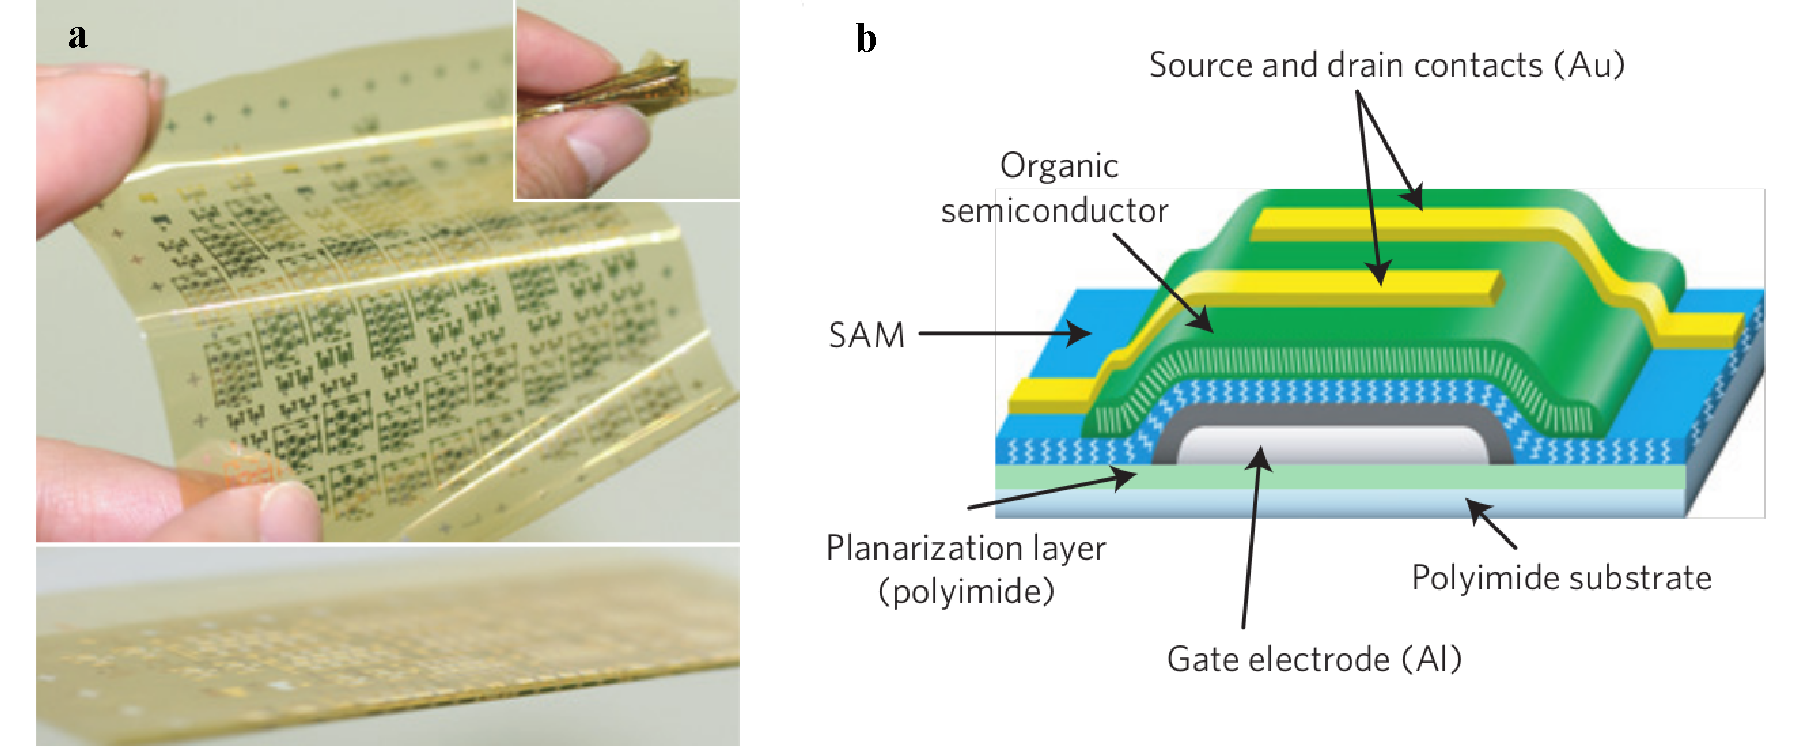
\includegraphics[scale=0.45]{Spintronique/MolecularElec/MolecularElec.pdf}
\caption{\textbf{a} : Photographie d'un substrat de polymide contenant des transistors organiques. \textbf{b} : Vue en coupe d'un transistor organique~(figure extraite de~\cite{Sekitani2010}).}
\label{MolecularElec}
\end{figure}


Depuis, de nombreux dispositifs issus de l'électronique moléculaire ont vu le jour, comme les  transistors à base de films fins organiques (ou OFTFs - cf Fig.\ref{MolecularElec}). Mais aucune application n'a, à ce jour, tiré partie de la taille nanométrique des molécules, et la route est encore longue avant l'obtention de dispositifs commerciaux ne mettant en jeux que quelques molécules, voire une seule.

Comme le rappelle les auteurs de~\cite{Gatteschi2006} , une conséquence plus inattendue du développement de l'électronique moléculaire est d'avoir participé à l'essor du magnétisme moléculaire, domaine que nous allons aborder maintenant.


\section{Le magnétisme moléculaire}
L'interêt réciproque entre l'électronique organique et le magnétisme moléculaire réside dans le fait que les aimants moléculaire sont de très bon candidat pour la résalisation de dispositifs de spintronique~\cite{Bogani2008,Sanvito2011}.La première raison à cela n'est pas propre aux aimants moléculaire mais vrai pour toute molécule : on sait le fabriqué en grande quantité, avec des propriétés contr\^olés et un grand degré de pureté.

\begin{figure}
\centering 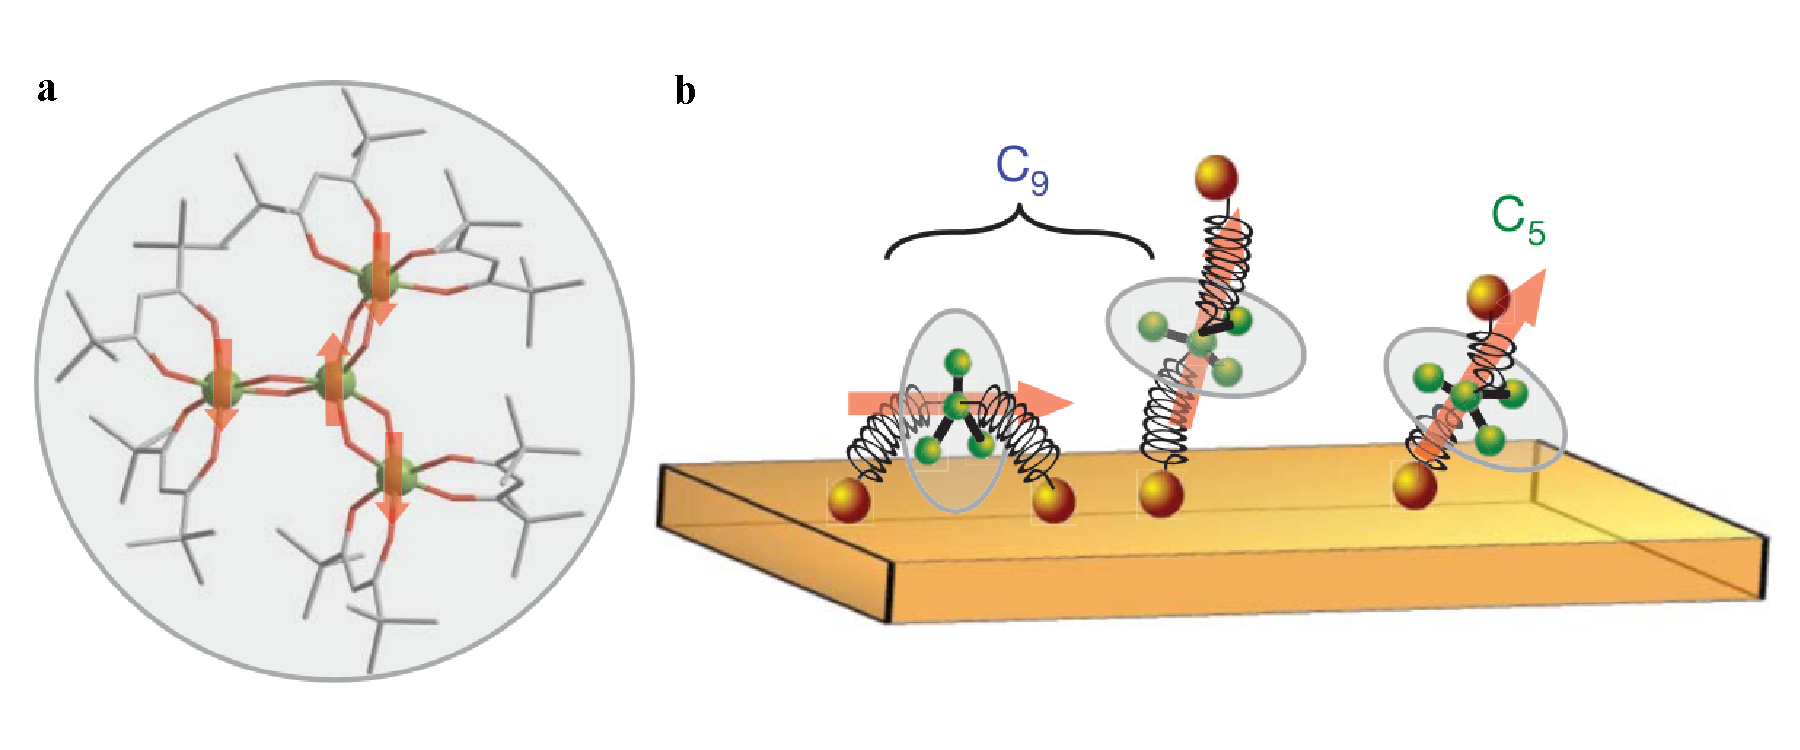
\includegraphics[scale=0.45]{Spintronique/MolecularMag2/MolecularMag2.pdf}
\caption{\textbf{a} : Structure du \textit{cluster} de Fe$_4$. \textbf{b} : Représentation des différent mode d'ancrage~(extrait de~\cite{Mannini2010}).}
\label{MolecularMag2}
\end{figure}

De plus, par l'ajout de ligand, les molécules peuvent s'auto-assembler pour former des structures parfois complexes, sans la mise en œuvre de techniques lithographiques conventionnelles. Récemment, l'équipe de Roberta Sessoli ont pu montrer qu'il était possible de contrôler la direction préférentielle de l'aimantation adopté par les SMM une fois sur la surface, par le choix de ligands adaptés. A l'aide du système obtenu, ils ont également mis en évidence le retournement de l'aimantation de molécule de Fe$_{4}$~\cite{Mannini2010}~(cf Fig.\ref{MolecularMag2}).

Par ailleurs, les aimant moléculaires, de par leur taille, représente la solution de stockage ultime. L'information pourrait être coder par l'orientation de leur moment magnétique, extrêmement stable à basse température, accroissant ainsi la capacité de stockage informatique.

En outre, il est possible de rendre leur magnétisme dépendant de stimulus extérieurs tels que la lumière ou bien encore la chaleur. De telles propriétés pourrait \^etre mise en oeuvre dans la fabrication de détecteurs, de mémoires, ou bien encore dans la conception de dispositifs opto-électronique.

Cependant, l'électronique conventionnelle n'est pas la seule possibilité d'application. En effet, le magnétisme moléculaire est régie par les lois de ma mécanique quantique. A ce titre, ils pourrait utilisé pour implémenté les fameux bit quantique ou qbit dans le cadre de l'information quantique. C'est notamment à l'investigation de ces propriétés que se consacre l'étude du magnétisme moléculaire.
 
Essayer de dresser un panel complet du magnétisme moléculaire est un travail complexe auquel je ne m'attacherai pas ici. Pour cela, je renvois le lecteur à~\cite{Gatteschi2006} et son excellente introduction. Je ne vais souligner ici que quelques étapes présentant certains des phénomènes physiques majeurs mis en évidence dans les aimants moléculaires.

La première mesure d'un effet quantique sur un aimant moléculaire~(SMM ou Single Molecular Magnet) a été obtenue en 1995 à partir d'un échantillon de poudre d'une molécule maintenant bien connue : le Mn$_{12}$Ac~\cite{Friedman1996}. Quelques temps plus tard, cette mesure était confirmée à l'aide d'un cristal moléculaire de Mn$_{12}$Ac~\cite{Thomas1996}. Cet effet quantique est connu sous le nom de retournement de l'aimantation par effet tunnel~(ou QTM - Quantum Tunneling of the Magnetization).

Celui-ci correspond au retournement de l'aimantation d'une molécule malgré la présence d'une barrière de potentiel entre les deux orientations opposées~(cf Fig.\ref{MolecularMag}.\textbf{a}). Ceci n'est possible que lorsque deux états du système, situés de part et d'autre du puits de potentiel, sont amenés en résonance à l'aide d'un champ magnétique. Le phénomène de QTM ne peut se faire que pour des valeurs de champ magnétique bien précises donnant lieux à des mesures de cycle d'hystérésis présentant des marches~(cf Fig.\ref{MolecularMag}.\textbf{b}).

\begin{figure}
\centering 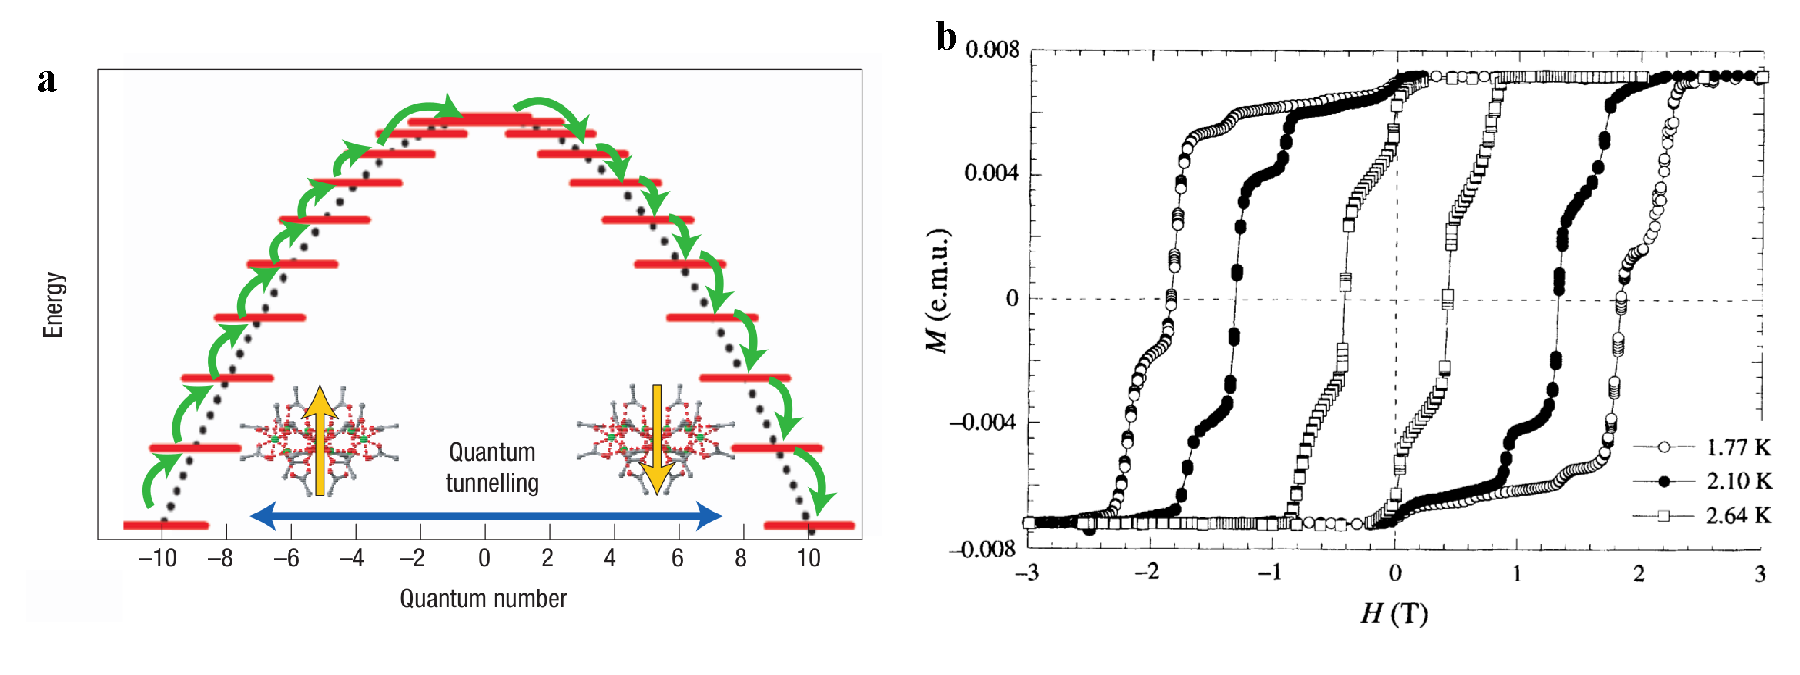
\includegraphics[scale=0.45]{Spintronique/MolecularMag/MolecularMag.pdf}
\caption{ \textbf{a} : Echelle des énergie des différant état de spin pour un spin $S=10$. Le renversement peut s'effectuer par effet tunnel~(QTM - Quantum Tunneling of the Magnetizion) lorsque un des niveaux dans le premier puit est en résonance avec un niveau dans le second~(flèche bleu). L'aimantation peut également ``monter" l'échelle des énergie par l'absorbtion de phonon pour ensuite redescendre dans le second puit en emmettant des phonons~(flèche verte)~(extrait de~\cite{Bogani2008}).\textbf{b} : Première mesure du phénomène de QTM sur un cristal moléculaire de Mn$_{12}$Ac~(extrait de~\cite{Thomas1996}).}
\label{MolecularMag}
\end{figure}

Trois ans plus tard, Wolfgang Wernsdorfer et Roberta Sessoli mettaient en évidence l'oscillation dans les probabilité de retournement par QTM dû à un effet quantique d'interférence semblable à la phase de Berry~\cite{Wernsdorfer1999}. Dans ce phénomène, les interférences se font entre le différents ``chemins" que l’aimantation peut prendre sur la sphère de Bloch lors de son renversement. Ceci se traduit par une variation dans les probabilités de retournement et donc, par une modulation de la hauteur des marches associés au QTM.

La structure hyperfine de certains terres rares a pu également être explorée. En effet, la position en champ des retournements par QTM peut être, dans certains cas, fortement influencé par l'état du spin nucléaire. Le TbPc$_{2}$, où Terbium Double-Decker~( en référence aux avions à deux ailes), a notamment été caractérisé en détail à l'aide de la technique micro-SQUID, et les paramètres de couplage hyperfin ont pu être extraits de la mesure de l'aimantation d'un cristal moléculaire~\cite{Ishikawa2005}. D'autre noyaux que le Tb ont également été analysés avec succès à l'aide d'une structure moléculaire identique~\cite{Ishikawa2005a}.

Mais les progrès de l'électronique moléculaire n'ont pas laissé la communauté du magnétisme indifférente et la question de l'interaction entre aimant moléculaire et surface métallique a commencé à se poser. Une étude portant sur une molécule de Mn$_{12}$ déposée sur une surface d'or a été réalisée en 2008~\cite{Mannini2008} en combinant différents moyens d'analyse~(XAS et XMCD). Elle conclue que la structure de l'aimant moléculaire est modifiée lorsque ce dernier est déposé sur une surface et que le magnétisme est également affecté. Cette fragilité a été confirmée par une seconde étude~\cite{Mannini2009} soulignant l'importance du choix du SMM pour les applications de spintronique moléculaire.

Cependant, une meilleure compréhension du magnétisme moléculaire et de ses interactions avec l’environnement passe par le développement de la spintronique moléculaire, seul moyen d'investigation à l'échelle de la molécule unique. C'est donc également dans cette voie que se sont engagé à la fois les chimistes et les physiciens comme je vais le présenter maintenant.


\section{La spintronique moléculaire}
La spintronique moléculaire a pour but de combiner les techniques de la spintronique avec les nouveaux développements de l'électronique moléculaire et de la chimie, afin de produire de nouveaux dispositifs susceptibles de compléter ou éventuellement remplacer les technologies tout semi-conducteurs déjà existantes. Cette discipline a connu une évolution rapide ces dernières années, bénéficiant des dernières avancés en matière de lithographie, mais aussi de la mise en synergie du travail des physiciens et des chimistes. 

Dans ce paragraphe, je ne présenterai bien sûr qu'une petite partie des nombreux travaux effectués dans le domaine. Ceci ne constitue donc en aucun cas une liste exhaustive des expériences réalisées, ni m\^eme une sélection des travaux les plus importants. Elle permettra, je l'espère, au lecteur de situer nos recherches par rapport à celles en cours dans d'autres laboratoires. De plus, je me limiterai ici aux dispositifs ne comportant qu'un nombre limité de molécules, de l'ordre de l'unité, généralement utilisés dans les laboratoires de recherche fondamentale.
\subsection{État de l'art}

\subsubsection*{Du premier transistor moléculaire...}
La première expérience de mesure de courant à travers une molécule unique a été réalisée en 1995 à l'aide d'un microscope à effet tunnel~\cite{Joachim1995}~(ou STM). Il s'agissait de mesurer la résistance à travers une molécule de C$_{60}$ déposée sur une surface d'or. Il n'était pas question d'obtenir un transistor, puisque seul deux terminaux étaient présents à savoir, la surface conductrice et la pointe du STM.

Cette expérience, et celles qui ont suivi, ont encouragé le développement de nouvelles techniques permettant de piéger une molécule unique dans un dispositif de mesure. C'est ainsi qu'est apparu la technique dite de``break junction"~\cite{Zhou1995}. Elle consiste à suspendre un fin pont métallique déposé sur un substrat flexible, puis à plier le support jusqu'à obtenir une cassure. La taille de celle-ci peut être ensuite modulée en faisant varier la courbure imposée à l'échantillon. A l'aide de ce dispositif, Reed \textit{et al.} ont pu mesuré, en 1997, des molécules de benzene-1,4-dithiol et étudié l'influence du couplage entre les électrodes et la molécule, sur la conductance mesurée~\cite{Reed1997}. Cette technique présente cependant l'inconvénient de ne pas pouvoir disposer d'une grille locale permettant de moduler le potentiel de la molécule.

\begin{figure}
\centering 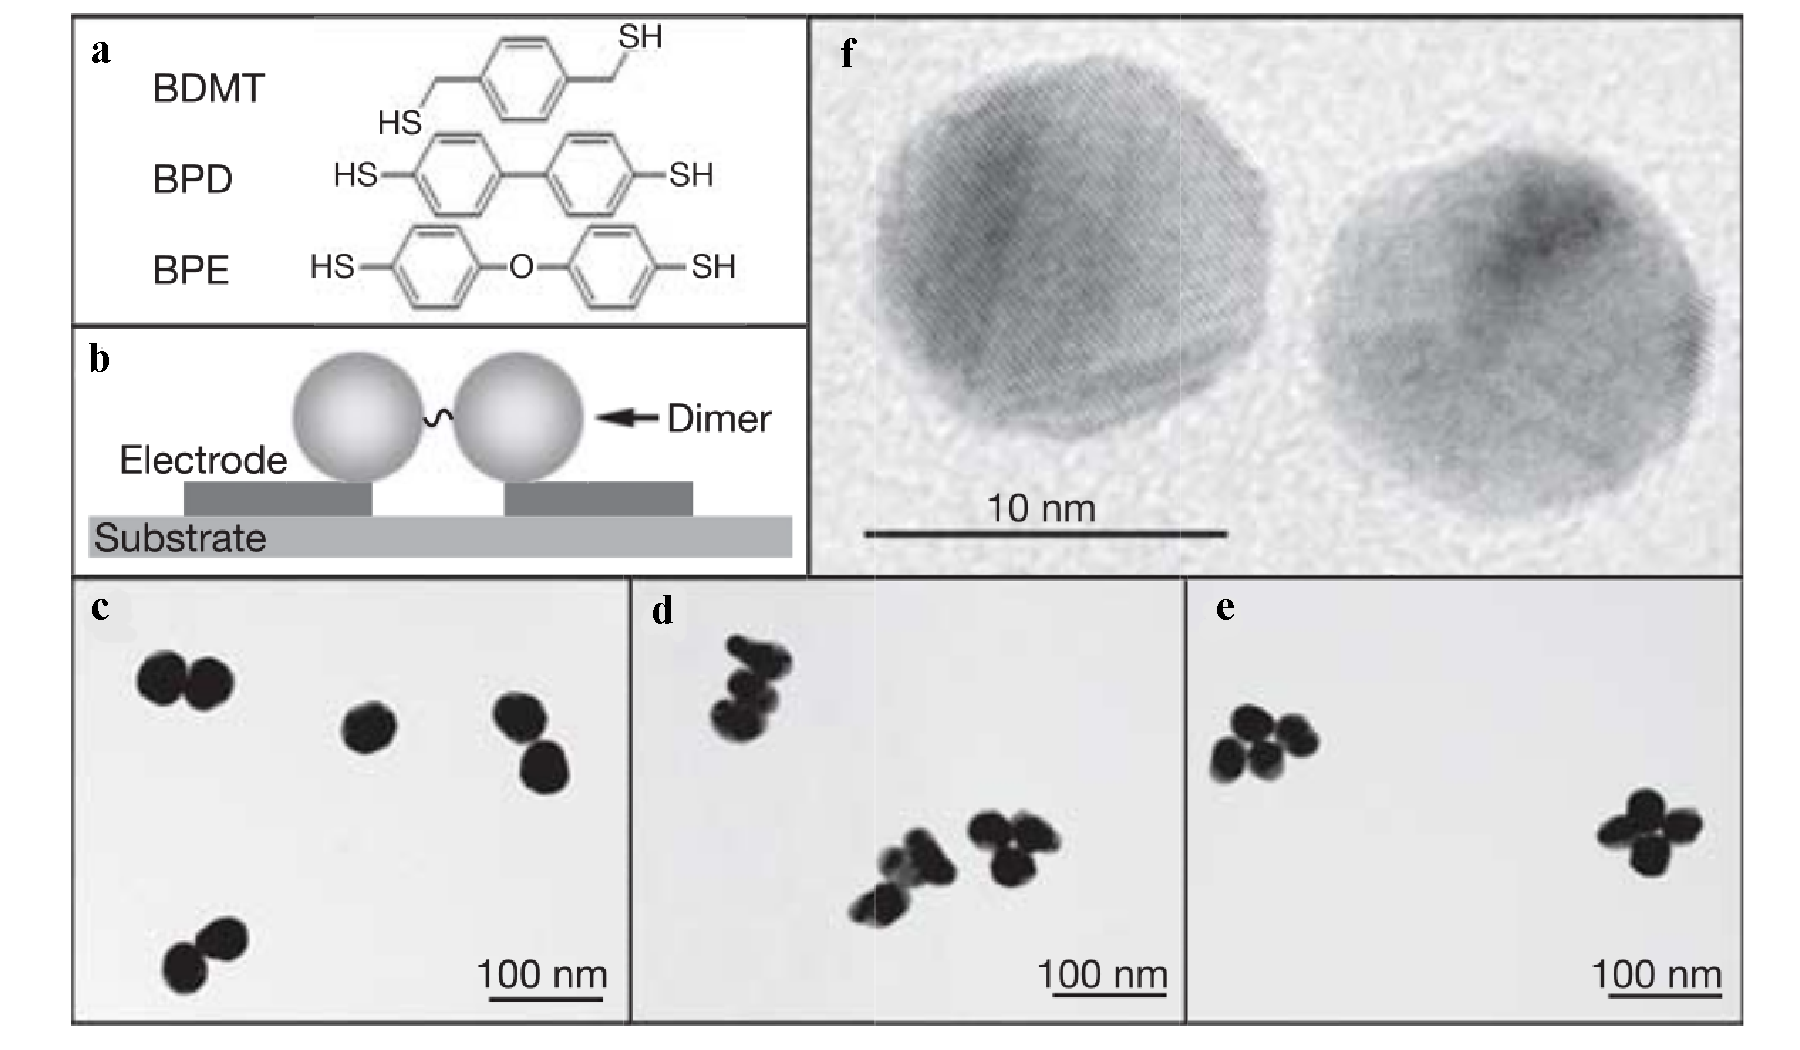
\includegraphics[scale=0.45]{Spintronique/MolSpintro2/MolSpintro2.pdf}
\caption{\textbf{a} : image obtenue par microscopie électronique à balayage d'une jonction moléculaire obtenue par technique d'électromigration, ainsi que la vue d'artiste correspondante~(extrait du site WEB de l'université de Tel Aviv). \textbf{b} : image par microscopie électronique à transmission~(TEM) d'un dimer à base de BDMT constitué par deux billes d'or de $10\,nm$. Le nanomètre qui sépare les deux billes correspond approximativement à la taille de la molécule de BDMT~($0.9\,nm$).Figure extraite de~\cite{Dadosh2005}. \textbf{c} : image par microscopie électronique à balayage d'une jonction à cassure~(image CEA/LEM). \textbf{d} : image d'artiste d'une mesure STM~(extrait de \cite{Leary2011}).}
\label{MolSpintro2}
\end{figure}


Pour pallier à cet inconvénient, il a fallu attendre encore 3 ans et la réalisation du premier transistor à molécule unique~\cite{Park2000}. Celui-ci consistait en un atome de C$_{60}$ piégé entre deux électrodes d'or déposé sur une grille. Ce dispositif a été obtenu en utilisant un phénomène bien connu des micro-électronicien, puisqu'à l'origine de nombreuse défaillance dans les dispositifs électroniques~\cite{Ho1989,Tu1992} : l'électromigration. Nous présenterons cette dernière en détail dans le chapitre consacré à la fabrication de notre échantillon.

L'expérience menée sur ce premier transistor moléculaire avait pu mettre en évidence le couplage entre les modes de vibrations moléculaires et les caractéristiques de transport à travers ce transistor à molécule unique. De plus, la grille se révélait suffisamment efficace pour modifier l'état de charge de la molécule de C$_{60}$ permettant ainsi d'obtenir les premiers diamants de Coulomb associé à une molécule unique.

Une étape supplémentaire a été franchie par le groupe de A. Yacoby~\cite{Dadosh2005}~(cf Fig.\ref{MolSpintro2}) Ils ont mis au point la première approche réellement ``Bottom-Up" en attachant chimiquement une molécule à deux billes d'or de quelques nanomètres, pour venir ensuite contacter ces dernières à l'aide de deux électrodes.\`A ma connaissance, cette technique n'a été réutilisée qu'une seule fois depuis~\cite{Jain2009}. Elle illustre néanmoins le rôle central que pourrait jouer la fonctionnalisation, dans une approche entièrement ``Bottom-Up".

Cependant, dans la grande majorité de ces dispositifs, aucune propriété propre aux molécules n'est utilisée et le seul spin en jeu dans les phénomènes observés reste celui de l'électron. Hors, l'avantage principal des molécules, outre leur taille, provient des différentes propriétés, notamment magnétique, que la chimie moderne peut leur conférer.

\subsubsection*{\`A la spintronique moléculaire}

L'année 2006 a vu paraître les deux premières expériences visant à insérer des aimants moléculaires au sein d'une interstice nanométrique afin d'obtenir les premiers dispositifs de spintronique moléculaire~\cite{Heersche2006,Jo2006}~(cf Fig.\ref{MolSpintro}). La première a été publiée par le groupe de H.S.J van der Zant et la seconde par le groupe de D.C. Ralph, et portaient toutes deux sur l'étude d'un aimant moléculaire bien connu : le Mn$_{12}$. Un des aspects intéressant de ces expériences, outre le magnétisme de la molécule, est la fonctionnalisation de cette dernière à l'aide de groupe thiol, afin de favoriser le couplage avec les électrodes d'or. Il illustre, encore une fois, la souplesse de la chimie et la possibilité qu'elle offre de fabriquer des molécules faites sur mesure, afin de faciliter certaines configurations ou certains comportements~(ici une forte affinité avec l'or).  

Cependant, les mesures en transport, bien que montrant une dépendance en champ magnétique complexe et des signes de conductance différentielle négative, n'ont pas permis de confirmer, de façon certaine, s'il s'agissait bien d'une molécule de Mn$_{12}$, ni même de savoir si les propriétés magnétiques de cette dernière avait été conservées durant la fabrication. Le groupe de D.C. Ralph conclue d'ailleurs ses travaux par la phrase suivante : ``\textit{We find significant variations between devices, indicating that the sample fabrication process and the device environment may affect our molecules}".

La première expérience réellement convaincante de transistors moléculaires mettant en jeu une molécule magnétique a été réalisée en 2008 dans le groupe de D.C. Ralph~\cite{Grose2008}. Toujours avec la technique d'électromigration, son équipe avait produit un transistor à base de N@C$_{60}$. Elle avait alors pu mettre en évidence, à travers des mesures en transport, le magnétisme lié à l'atome d'azote de spin S=3/2,  et remonter au couplage entre ce dernier et les électrons de la cage de C$_{60}$. 

\begin{figure}
\centering 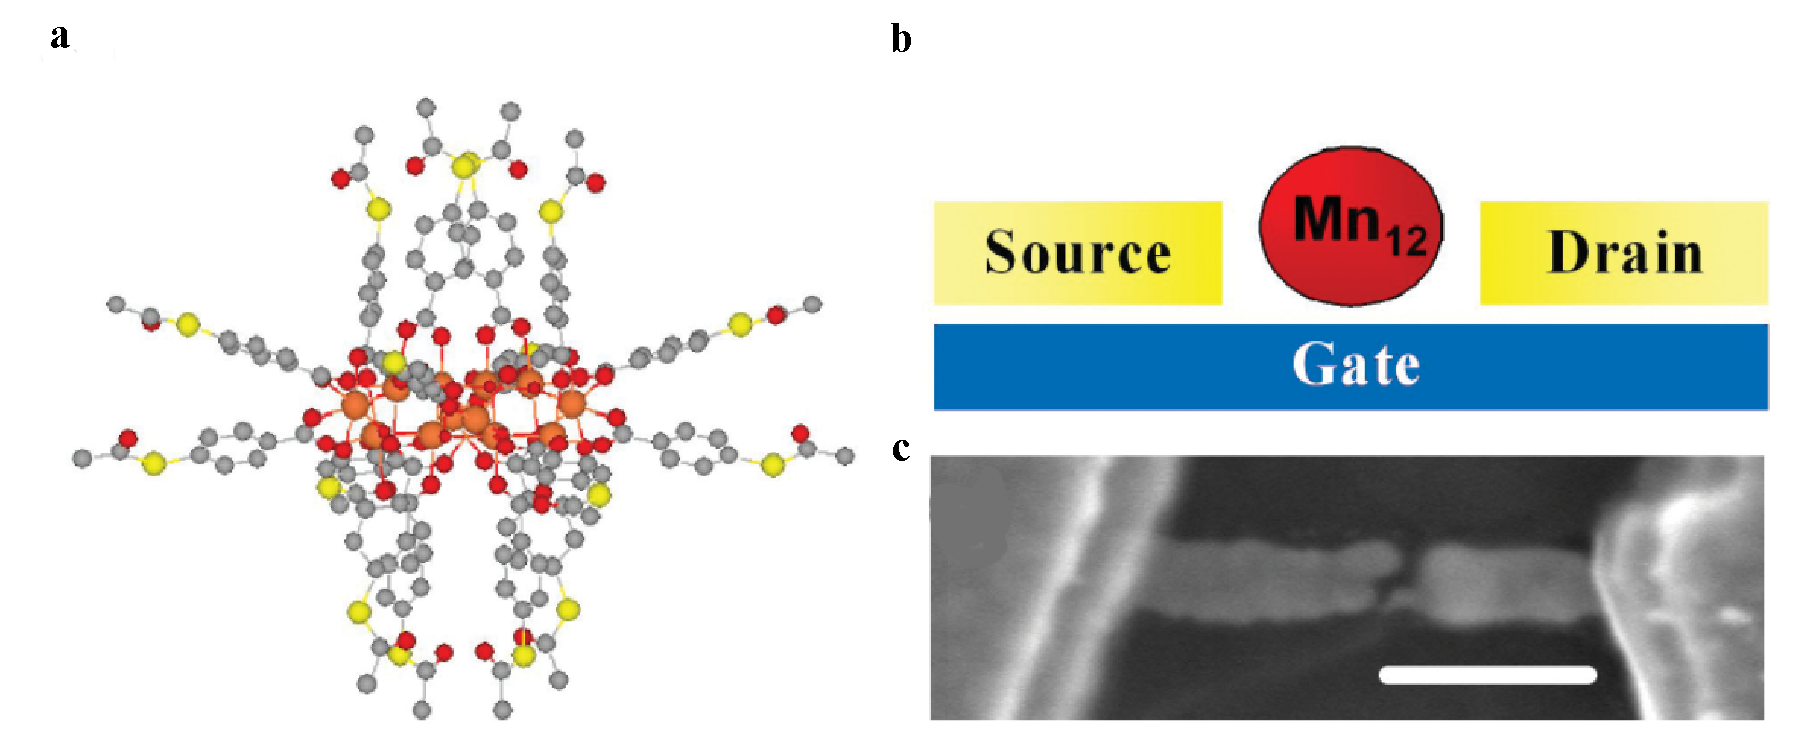
\includegraphics[scale=0.45]{Spintronique/MolSpintro/MolSpintro.pdf}
\caption{\textbf{a} : Structure du Mn$_{12}$ entouré de ligands thiols favorisant l'ancrage. \textbf{b} : Représentation schématique de la molécule de Mn$_{12}$ piégée entre les électrodes. \textbf{c} : Image de la jonction obtenue par microscopie électronique. Le trait blanc correspond à $200\,nm$.~(extrait de~\cite{Heersche2006}).}
\label{MolSpintro}
\end{figure}

Il s'agit, à mes yeux, du premier dispositif que l'on peut qualifier de spintronique moléculaire à l'échelle de la molécule unique. En effet, les propriétés magnétiques de la molécule isolée se retrouvent de façon non-équivoque dans les mesures en transport. Ce n'est d'ailleurs pas surprenant car, fort de leur expérience avec le Mn$_{12}$, les auteurs avaient choisi le N@C$_{60}$ pour la robustesse de sa structure et de ses propriétés magnétiques, comme ils le précisent dans leur papier. 

Cependant, bien qu'ayant un moment magnétique, cette dernière n'appartient pas à la catégorie des aimants moléculaires. En effet, elle ne possède pas d'anisotropie dans l'orientation de son moment magnétique, donc celle-ci n'est déterminé que par le champ magnétique appliqué. Il est donc impossible d'observer dans cette molécule, les phénomènes quantiques présentés dans le cadre du magnétisme moléculaire.

Loin d'\^etre des échecs, ces différents travaux ont fournis un apport important au reste de la communauté notamment concernant les critères essentiels que doivent remplir les aimants moléculaires susceptibles d'être étudiés par les techniques expérimentales actuelles. Je détaillerai ces différents critères lorsque j'introduirai le Terbium double-Decker.
 
\subsection{La spintronique dans notre groupe}
Le groupe au sein duquel j'ai effectué ma thèse a une culture ancrée dans le nano-magnétisme et le magnétisme moléculaire. Une bonne partie des efforts de la fin des années 1990 et du début des années 2000 a été consacré à l'analyse et la caractérisation de systèmes magnétiques allant de la nanoparticule au cristal moléculaire  et plus récemment, l'aimant moléculaire isolé et le spin nucléaire unique. A chaque échelle de moment magnétique correspond un dispositif de mesure, et assez logiquement, plus le moment magnétique à mesurer est faible, plus le détecteur est petit. Cette tendance est bien représentée dans la Fig.\ref{Group1}. Pour des particules macroscopiques, l'usage d'un SQUID est suffisant. Lorsque l'on veut caractériser des particules de l'ordre de quelques dizaines de nanomètre ou bien encore un cristal moléculaire, correspondant à des moments magnétiques de l'ordre de quelques milliers de $u_B$, l'usage d'un détecteur aussi sensible qu'un micro-SQUID est indispensable.


\begin{figure}
\centering 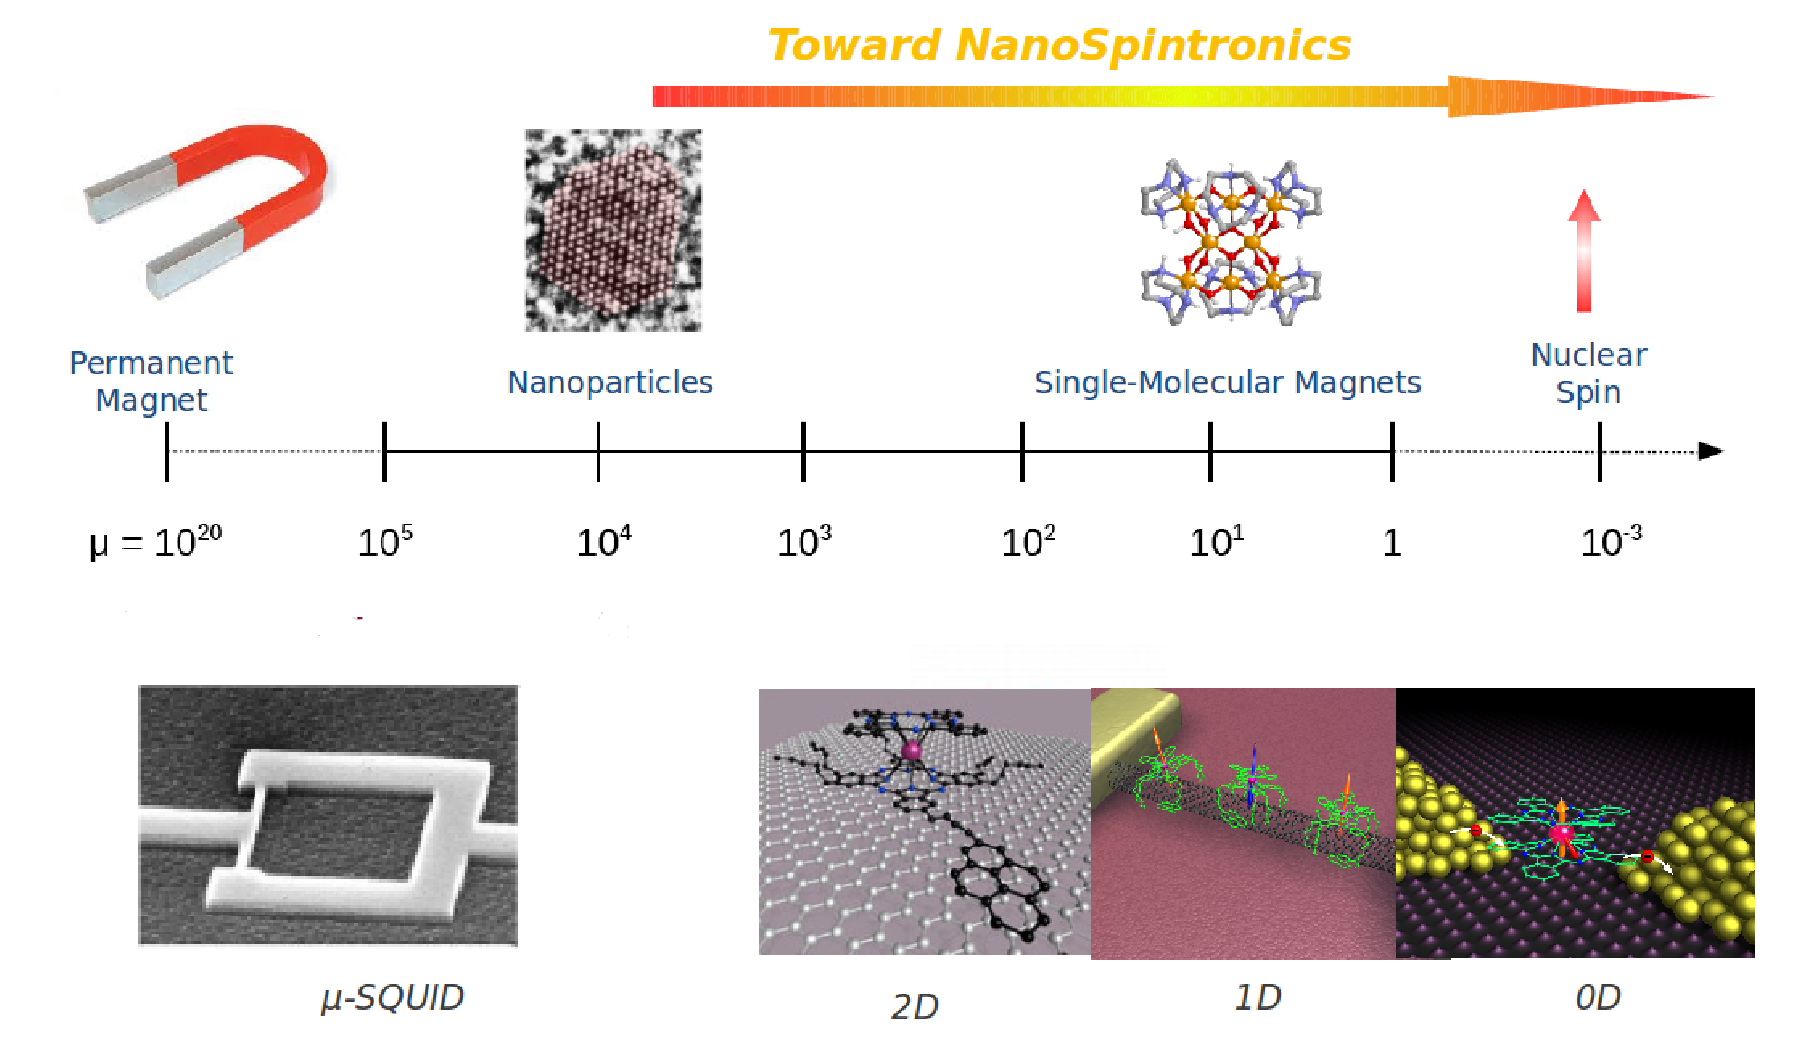
\includegraphics[scale=0.45]{Spintronique/Group1/Group1.pdf}
\caption{\'Evolution des dispositifs de détection en fonction de l'intensité du moment magnétique à mesurer.}
\label{Group1}
\end{figure}



Lorsque le moment magnétique a détecter devient très petit, de l'ordre du magnéton de Bohr, comme une molécule par exemple, il n'est plus vraiment possible de faire la distinction entre le détecteur et l'objet à mesurer. Il faut alors songer à fabriquer un dispositif électronique dont le fonctionnement même est influencé par le magnétisme de l'un de ses composants. Autrement dit, il faut faire appel à la spintronique et plus précisément, lorsque l'on s'intéresse aux molécules, à la spintronique moléculaire.

C'est dans ce cadre que se sont effectués les travaux conduisant à la fabrication du premier nanosquid en 2006~\cite{CleuziouJ.-P.2006}, dont les deux liens faibles supraconducteurs sont constitués par un nanotube. En outre, à l'aide de nanotube de carbone rempli de nanoparticule magnétique, une astroide de Stoner–Wohlfarth~\cite{Cleuziou2011} a été obtenue pour la première fois par des mesures en transport électronique. Dans ce dernier dispositif, l'objet à mesurer faisait parti intégrante du système de détection.

La thématique des nanotubes ne s'est pas arrêtée aux nanoparticules,et de nouveaux dispositifs à base d'aimants moléculaires ont été développés. Ils ont donné des résultats encourageants comme dans le cas de la vanne de spin obtenue par Matias Urdampilleta~\cite{Urdampilleta2011}. Dans son expérience, un tube a été relié à deux électrodes, une grille permettant de faire varier son potentiel. Un solution contenant des molécules de TbPc$_{2}$ a ensuite été déposée, puis l'échantillon a été disposé dans un frigo à dilution. Les résultats ont mis en évidence un comportement de type vanne de spin et une analyse fine des mesures a permis de déterminer que les rôles de polariseur et d'analyseur étaient joués par deux aimants moléculaires. Il s'agit là du premier dispositif de spintronique moléculaire mettant en jeux des aimants moléculaires. Il est assez amusant de constater que le premier dispositif qui a permis de mettre la spintronique sur le devant de la scène soit également la premier a être réalisé en spintronique moléculaire.

\begin{figure}
\centering 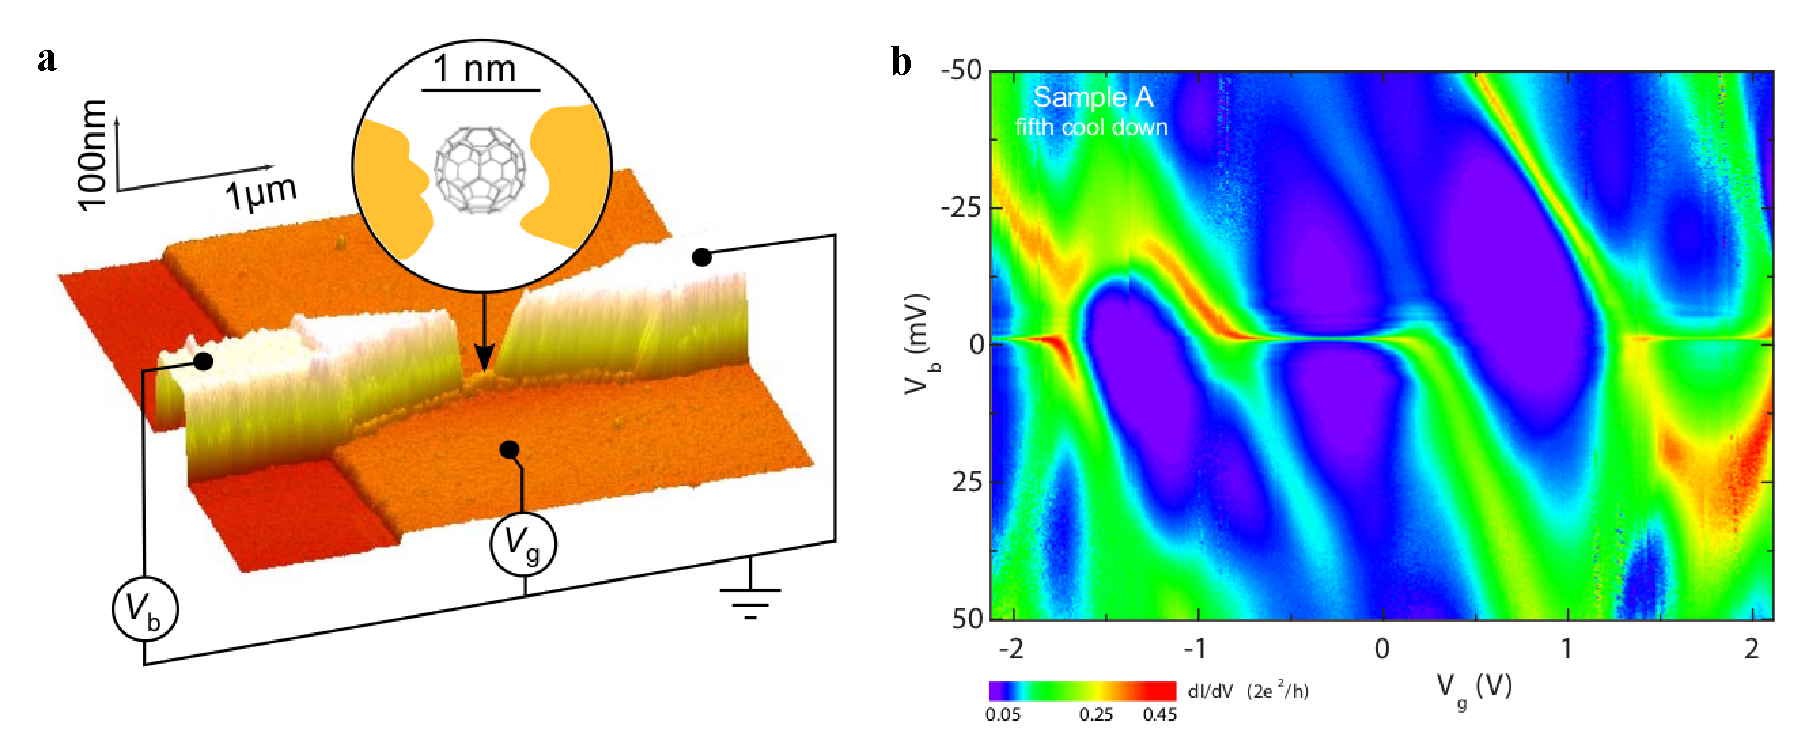
\includegraphics[scale=0.45]{Spintronique/RochC60/RochC60.pdf}
\caption{\textbf{a} : image obtenue par microscopie électronique à balayage illustrant la géométrie d'un transistor moléculaire obtenu par électromigration. \textbf{b} : spectroscopie en cotunneling en conductance différentielle de l'échantillon en fonction de la tension soure-drain $V_b$ et du champ magnétique $B$ pour une tension de grille $V_g$. \textbf{c} : vue d'artiste de la molécule de N@C$_{60}$. \textbf{d} : configuration magnétique de cette dernière en fonction de son état de charge~(extrait de \cite{Roch2011}).}
\label{RochC60}
\end{figure}


Afin d'améliorer encore la sensibilité de nos dispositifs, nous nous sommes intéressés à la fabrication de transistors à molécule unique. Pour cela, notre groupe a développé, à partir des travaux de H. Park~\cite{Park1999}, sa propre technique d'électromigration basée sur une boucle de contre-réaction rapide. Ces travaux ont d'abord permis la réalisation d'un transistor moléculaire à base de C$_{60}$. Celui-ci à conduit à l'observation de nombreux phénomènes quantiques tels que l'effet Kondo sous-écranté~\cite{Roch2009} ou bien encore la transition de phase quantique~\cite{Roch2008}. Puis, en collaboration avec W. Harneit, nous avons étudié la molécule de N@C$_{60}$~\cite{Roch2011}, confirmant les résultats obtenus quelques temps plus tôt par D.C. Raplh et complétant ses observations par des mesures en cotunneling. L'ensemble de ces travaux peut être trouvé dans la thèse de Nicolas Roch.

%\begin{figure}[H]
%\centering \includegraphics[scale=0.45]{Spintronique/Group2/Group2.pdf}
%\caption{Vue d'artiste de la vanne de spin moléculaire~(\textbf{a}) et du transistor moléculaire~(\textbf{b}) à base de TbPc$_{2}$.}
%\label{Group2}
%\end{figure}

Cette analyse nous a également permis d'identifier les faiblesses de notre dispositif expérimental. Il nous fallait ajouter deux axes magnétiques pour explorer les trois directions de l'espace, mais également être capable de balayer le champ beaucoup plus rapidement : avec des vitesses de plusieurs centaines de milli-Tesla par seconde. Fort de l'expérience du groupe dans le domaine du nanomagnétisme, un dispositif mettant en jeux deux bobines de faible inductance et un système de dilution rotative a été développé rapidement au sein du laboratoire. Ce dispositif a permis d'obtenir les résultats que je vais vous présenter dans cette thèse.

